\documentclass[10pt,portuguese,notheorems,compress]{beamer}

\usepackage{amsfonts,amsmath,amssymb,amstext,amscd,bezier}
\usepackage[scaled=.92]{helvet}
\usepackage[brazil]{babel}
\usepackage[utf8]{inputenc}
\usepackage[T1]{fontenc}
\usepackage{amssymb}
\usepackage{listings}
\usepackage{beamerthemesplit}
\usepackage{color}
\usepackage{amsfonts}
\usepackage{amsmath}
\usepackage{indentfirst}
\usepackage{setspace}
\usepackage{float}
\usepackage{amsmath,amsfonts}
%\usepackage[brazil]{babel}
%\usepackage[latin1]{inputenc}
\usepackage{graphicx}
\usepackage{ragged2e}
\usepackage{caption}
\usepackage{subcaption}

\newcommand{\pr}{\hspace*{0.6cm}}
\newcommand{\vesp}{\vspace*{.3cm}}
\newcommand{\sen}{\mbox{sen }}
\newcommand{\tg}{\mbox{tg}}
\newcommand{\Sum}{\displaystyle\sum}
\newcommand{\Prod}{\displaystyle\prod}
\newcommand{\Int}{\displaystyle\int}
\newcommand{\Lim}{\displaystyle \lim}
\newcommand{\Frac}{\displaystyle\frac}
\newcommand{\Dparc}[2]{\dfrac{\partial #1}{\partial #2}}
\newcommand{\Dparcn}[3]{\dfrac{\partial^#3 #1}{\partial^#3 #2}}
\newcommand{\R}{\mathbb{R}}
\newcommand{\V}{\mathcal{V}}
\newcommand{\I}{I_u}
\newcommand{\Fi}{\varphi}
\newcommand{\se}{\mbox{ se }}
\newcommand{\norma}[2]{\left\vert\left\vert #1 \right\vert\right\vert_{#2}}

\newtheorem{defi}{\pr \sc Defini\c{c}\ão}[section]
\newtheorem{obs}{\pr \sc Observa\cao}[section]
\newtheorem{teor}{\pr \sc Teorema}[section]
\newtheorem{lema}{\pr \sc Lema}[section]
\newtheorem{prop}{\pr \sc Proposi\cao}[section]
\newtheorem{exercise}{\pr \sc Exerc\'\i cios}[section]
\setlength{\columnsep}{1cm}
\newtheorem{definicao}{Defini\c c\ão}
\newtheorem{teorema}[definicao]{Teorema}
\newtheorem{corolario}[definicao]{Corol\'ario}
\newtheorem{exemplo}[definicao]{Exemplo}


\usetheme[secheader]{Boadilla}

\setbeamercovered{highly dynamic}
\usefonttheme{structurebold}
\usecolortheme{dolphin}

\renewcommand{\lstlistingname}{Arquivo }

\setbeamercolor{block title}{use=structure,fg=white,bg=black!35!blue}
\setbeamercolor{block title alerted}{use=alerted text,fg=white,bg=black!35!blue}
\setbeamercolor{block title example}{use=example text,fg=white,bg=black!35!blue}
\setbeamercolor{block body}{parent=normal text,use=block title,bg=block title.bg!10!bg}
\setbeamercolor{block body alerted}{parent=normal text,use=block title alerted,bg=block title alerted.bg!10!bg}
\setbeamercolor{block body example}{parent=normal text,use=block title example,bg=block title example.bg!10!bg}

\lstset{language=C++,
                basicstyle=\ttfamily,
                keywordstyle=\color{blue}\ttfamily,
                stringstyle=\color{red}\ttfamily,
                commentstyle=\color{green}\ttfamily,
                morecomment=[l][\color{magenta}]{\#}
}


\author{Adams, Ana, Fred}
\title{Torres de Hanói}
\institute{USP-ICMC}
\date[Apresentação]{Apresentação}




\begin{document}
\justifying

\begin{frame}
\begin{center}
	UNIVERSIDADE DE SÃO PAULO – USP
	
	INSTITUTO DE CIÊNCIAS MATEMÁTICAS E DE COMPUTAÇÃO
	
	DEPARTAMENTO DE SISTEMAS DE COMPUTAÇÃO
	
	\vspace{1cm}
	
	\Large{\textbf{TORRES DE HANÓI}}
	
	\vspace{1cm}
	
    \textbf{Alunos:}\\
	Adams Vietro Codignotto da Silva - $6791943$ \\ 
    Ana Clara Kandratavicius Ferreira - $7276877$\\
    Frederico Facco - $8532206$\\
	 
	\vspace{.7cm}
	
	São Carlos
	
	2014
\end{center}
\end{frame}
\section{Introdução}
\begin{frame}
\frametitle{Introdução}
Neste trabalho, iremos resolver o famoso problema das Torres de Hanói, utilizando uma representação em grafo e técnicas aprendidas em IA.
\end{frame}
\section{Modelagem do Problema}
\begin{frame}
\frametitle{Modelando o problema}
A meta é obter o número mínimo de movimentos. O número mínimo pode ser obtido utilizando recorrência.

Tomando \textit{n} como número de discos, \textit{a}, \textit{b} e \textit{c} como os pinos e $H(n,a,b,c)$ como a quantidade de movimentos para passar do pino \textit{a} para o pino \textit{b}, utilizando o auxiliar \textit{c}, temos:
\begin{equation}
\nonumber
\begin{array}{l}
H(1,a,b,c) = 1 \quad (a \rightarrow c)\\
H(n,a,b,c) = H(n-1,a,b,c), \quad (a \rightarrow b), H(n-1,c,b,a)
\end{array}
\end{equation}
\end{frame}

\begin{frame}
Podemos dizer então que para um número \textit{n} de discos, podemos gerar uma árvore contendo todas as possibilidades, com $3^n$ nós.
\begin{figure}[H]
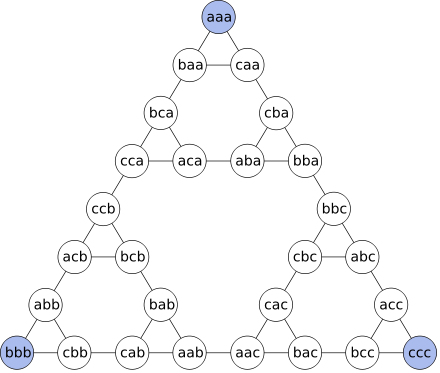
\includegraphics[scale=0.5]{1.png}
\caption*{\small{Árvore de possibilidades com 3 discos}}
\end{figure}
\end{frame}

\subsection{Recorrência}
\begin{frame}
Podemos dividir o problema da Torre de Hanói de acordo com o número de discos:
\begin{itemize}
\item Para n=1, basta 1 movimento
\item Para n=2, precisamos de 3 movimentos (trivial)
\item Para n=3, podemos resolver o problema para 2 discos (3 movimentos), mover o disco maior para o pino restante (1 movimento), e movemos os outros 2 discos para o pino final (3 movimentos) totalizando 7 movimentos.
\item Para n=4, Resolvemos o problema para três discos(7 movimentos), depois movemos o maior disco (1 movimento), após isso trazemos os três discos que já estão no outro pino para cima do maior disco (7 movimentos), totalizamos 15 movimentos.
\end{itemize}
\end{frame}

\begin{frame}
Podemos perceber que temos a seguinte seqüencia:
\begin{itemize}
\item $1=2^1 -1$
\item $3=2^2 -1$
\item $7=2^3 -1$
\item $15=2^4 -1$
\end{itemize}
Ou seja, temos $2^n-1$ movimentos necessários para uma quantidade \textit{n} de pinos.
\end{frame}
\section{Implementação}
\begin{frame}[fragile]
\frametitle{Implementação}
Utilizando a árvore de possibilidades, podemos utilizar a seguinte estrutura:

\begin{minipage}[b]{0.5\textwidth}
\begin{figure}[thp] % the figure provides the caption
\centering          % which should be centered
\begin{tabular}{c}
\
\begin{lstlisting}[tabsize=8,language=C++]
typedef struct grafo{
   int key[20];
   int flag;
   Lista *L;
}Grafo;
\end{lstlisting}
\end{tabular}
\caption*{Estrutura do Grafo}
\end{figure}
\end{minipage}%
\begin{minipage}[b]{0.5\textwidth}
\begin{figure}[thp] % the figure provides the caption
\centering          % which should be centered
\begin{tabular}{c}
\begin{lstlisting}[tabsize=8,basicstyle=\ttfamily]
typedef struct bloco {
        int valor;
        int flag;
        struct bloco *prox;
} no;
typedef struct {
        no *inicio;
        no *fim;
} Lista;
\end{lstlisting}
\end{tabular}
\caption*{Estrutura da lista de Adjacência}
\end{figure}
\end{minipage}%
\end{frame}

\begin{frame}
\frametitle{Algoritmos de busca}
Utilizamos inicialmente as buscas \textit{DFS (Depth-first Search, Busca em Profundidade)} e \textit{BFS (Breadth-first search, Busca em Largura)} como buscas cega. Podemos percorrer o grafo pelo lado esquerdo, chegando sempre à solução ótima.

Porém, como se trata de uma busca cega, a DFS irá chegar ao resultado ótimo, enquanto a BFS irá percorrer muito mais nós.
\begin{figure}[H]
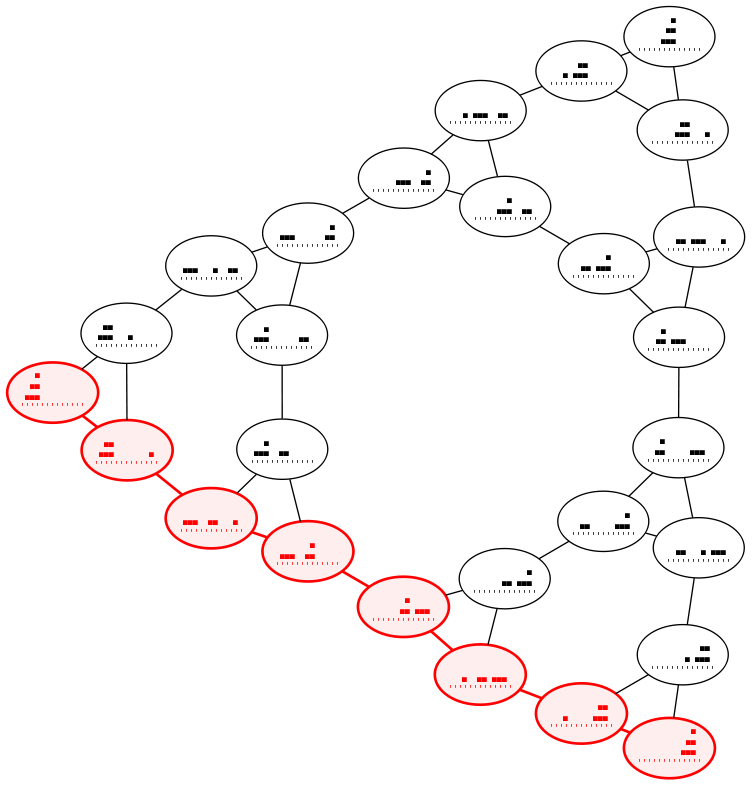
\includegraphics[scale=0.2]{2.png}
\end{figure}
\end{frame}
\section{Heurísticas}
\begin{frame}
\frametitle{Heurísticas}
Para o Algoritmo A*, usamos as heurísticas:
\begin{itemize}
\item Um contador de movimentos, onde a cada estado que passamos é incrementado.
\item A distância do estado até o estado desejado, onde o peso atribuído ao nó é a quantidade de discos que ainda não estão na posição final (no terceiro pino)
\end{itemize}
\end{frame}

\begin{frame}
Para o algoritmo A*, dado um vértice inicial v, e seja $d_{min}$ a distância total mínima, mantenha uma fila de prioridades (ou uma pilha) de nós a serem visitados, ordenado em ordem decrescente de custo:
\begin{enumerate}
\item Retire o primeiro elemento da fila e some o peso do elemento ao peso de seus vizinhos.
\item Reinsira os vizinhos na fila.
\item Se a distancia até o estado final for maior que a distância atual, a distância nova é a distância atual para o vértice v.
\item Continue até encontrar o alvo ou até que não tenha mais elementos na fila.
\end{enumerate}
Todos os nós devem manter um histórico de seu predecessor para que futuramente possa ser resgatado o menor caminho possível até o alvo.
\end{frame}
\begin{frame}
\frametitle{Análise dos Algoritmos}
\begin{center}
\begin{table}[H]
\begin{tabular}{|c|c|c|c|c|}
\textbf{Número de Discos} & \textbf{BFS} & \textbf{DFS} & \textbf{A*} & \textbf{Ideal} \\
\hline
1 & 1 & 1 & 1 & 1 \\
2 & 6 & 8 & 3 & 3 \\
3 & 24 & 26 & 8 & 7\\
4 & 70 & 74 & 15 & 15\\
5 & 232 & 220 & 25 & 24\\
\end{tabular}
\end{table}
\end{center}
Note que: A* necessita de mais memória que DFS e BFS juntos.
\end{frame}
\end{document}